\subsection{Physics-Informed Neural Network: Introduction}


\begin{wrapfigure}{r}{0.4\textwidth} % 'r' for right alignment, 0.4\textwidth for image width
    \centering
    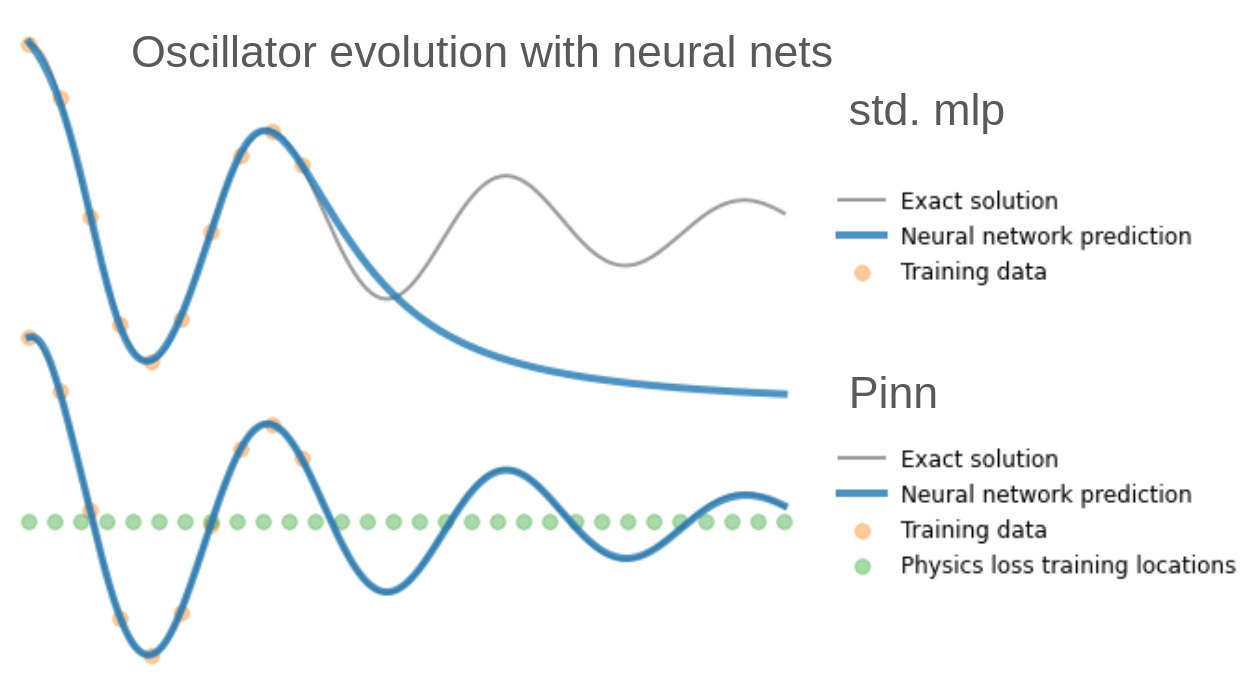
\includegraphics[width=\linewidth]{assets/oscillator.jpg} % Replace with your image file
    \caption{Example of the Pinn behavior.}
\end{wrapfigure}

Traditional methods for solving differential equations, such as finite element or finite difference methods, often require discretization of the domain and can be computationally expensive for high-dimensional problems.
Physics Informed Neural Networks (PiNNs) propose an alternative approach where the solution is approximated by a neural network that is trained not only on data but also by enforcing the underlying physical laws via the differential equations.
This approach should be able to generalize outside the training data, fully respect the underlying physics. 
With outside training data, we intend to say that the model generalize for sample that has never been shown \textbf{inside} the range of training. 
\\ 

The main loss component of the Pinn is called Physics Loss, and minimize the discrepancy between the dynamics of the system and the derivative of the network itself. 

The standard PiNN models takes in input just the time $t$ at which we want to predict the evolution of the system. So, the output of the model is define as $x(t)$.
For impose particular constraints, other losses are taken into account. Example of such loss are the so call \textit{Boundary loss} and the \textit{Initial loss}. 
The first one is used to impose the boundary condition of the system, while the second one is used to impose the initial condition of the system.
\\

One limitation of such approach is that the model is not able to generalize to different initial condition: the model need to be trained again for predict a new evolution. 
Also, as few works have shown, the classica formulation of the Pinn is not stable over long time interval. 
Finally, the standard pinn model is not able to include the control input into the dynamics. 

For this reason, we have used a extended version of the framework, namely, the PiNN-C (\textit{PiNN with control} \cite{Antonelo_2024}).
Such works shown as incorporate the control input on the prediction scheme, and has became the de-facto standard for model non-autonomus dynamic evolution (\cite{pinn-manipulators} \cite{ramp-net}).
The Pinn-C model is analyze in the next section of this report.

\subsection{Physics-Informed Neural Network with Control}


The Pinn-c framework rely on the assumption that the input is constant over a sub-interval $[0, T_k]$.
This assumption is used for ensure that the gradient of the output is not "corrupted" by the derivative of the state respect the input signal. 
In this framework, the input of the network is composed by the initial condition of the sub-transition, the time stamp for which we want to obtain the prediction and the constant control input.
Doing so, we obtain a set of tuple of the form $\left\{[x_{0}, \bar{u_{k}}, t_k], [x_{t_k}]\right\}$, where $x_{0}$ is the initial state of the system, $t_{k}$ is the time stamp for which we want to predict the evolution and $\bar{u_{k}}$ is the control input applied to the system.

The pinn-c, in the ground, just model a set of smaller evolution, and the discriminative factor remains the time input, as in the standard formulation.  

\begin{figure}[h]
    \centering
    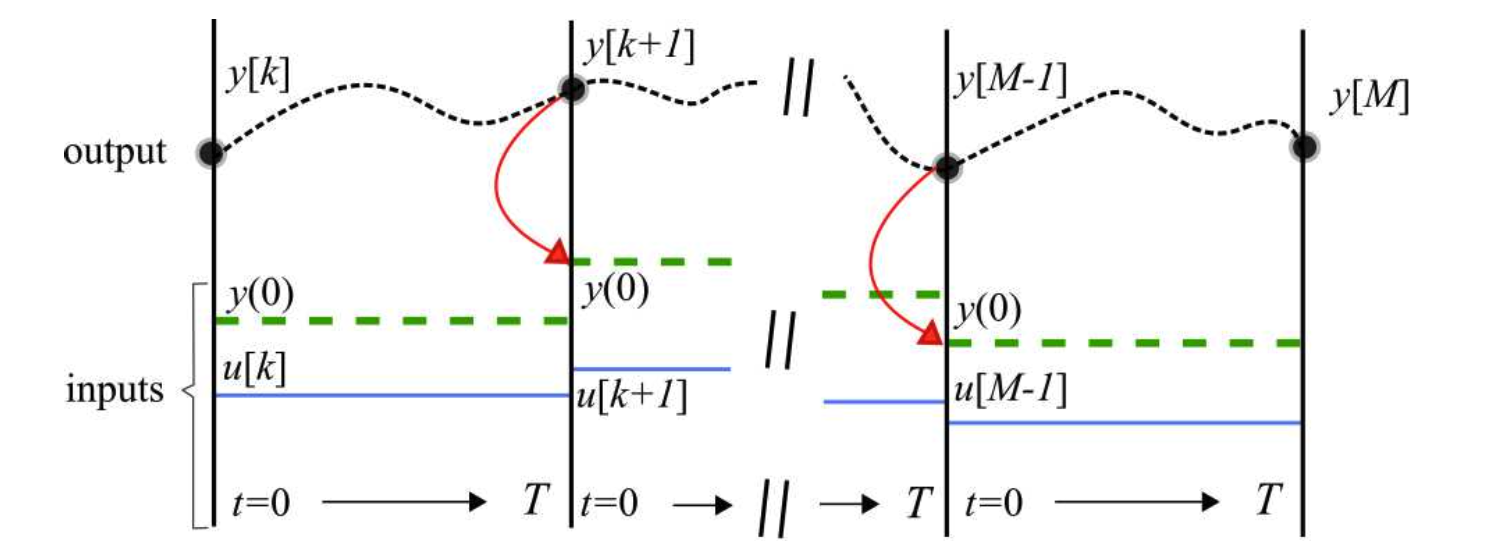
\includegraphics[scale=0.5]{assets/pinc_time.png}
    \caption{Pinn-c sub-interval integration}
    \label{sub-transition-integration}
\end{figure}

For concatenate the sub-trajectories, the starting continion of the next sub-trajectory is setted as the output of the previous interval at time $T$. For a concise representation, see figure \ref{sub-transition-integration}
Finally, while the standard pinn can not rely on the trajectories from a dataset, the pinn-c must use it. This dependency is modeled as a imitation loss, similar to the standard MLP case. 
\\
In such framework it's not possible to rely on multi-step integration for calculate the loss term. Due the definition of input/output of the network, it's impossible to concatenate the previous integration into the future input.
Extra details on the loss are given on the section below. 


\subsubsection{Dataset requirements, generation and constraints}

In our experiment, after generate the evolution of the system, we notice that a good converage of the input space of the network is required.
In the first phase of the experiment, we have generated a set of trajectories using a fixed family of input, like sinusoidal or step function. 
Although good result in the training and in the evaluation of the model (isolated form the mpc), we have notice that several phenomena conflict with the integration of the network into the mpc.
In particular, the network was not able to predict the evolution of the system when the control input was null. Also, basic motion like forward or backward trajectories remains challenging.

For this reason, we have decided to generate a new dataset, where the control input is randomly generated but all the possible combination of sing of the input are taken into account:
we have generated 8 different combination for the Unicycle:
\begin{multicols}{2}
    \begin{itemize}
        \centering
        \item $v > 0, w > 0$
        \item $v > 0, w < 0$
        \item $v < 0, w > 0$
        \item $v < 0, w < 0$
        \item $v > 0, w = 0$ 
        \item $v < 0, w = 0$
        \item $v = 0, w > 0$
        \item $v = 0, w < 0$
    \end{itemize}
\end{multicols}

The last possible combination, $v = 0, w = 0$, has been excluded from the dataset, as we model a additional loss term that relies on sampling.
The dataset has been generated using a Runge-Kutta 4th order method, and the sub-interval has been set to $0.1$ seconds. In order to approximate the real evolution of the system, 
the PiNN-C framework needs different sample in which the input is constant. For this reason, after having discretize the input signal, we have taken up to 10 sub-evolution, leading to a reading of the trajectory of $0.02$ seconds.

Under this assumption and constraint, we have seen that the previously mentioned phenomena are no longer present or at least has been minimized under a significant threshold.

\subsubsection{Loss definition and training scheme}

The overall loss function $\mathcal{L}$ used is composed by the sum of two main terms, which are the data loss (also call \textit{imit loss}) $\mathcal{L}_{data}$ and the physics loss $\mathcal{L}_{phy}$. 
\begin{equation}
    \mathcal{L}(\theta) = \mathcal{L}_{\text{data}}(\theta) + \mathcal{L}_{\text{phy}}(\theta),
\end{equation}

The first term defines the discrepancy between the prediction of the network and the observed data, while the second one specifies the correct modeling of the differential equation.
Usually $\mathcal{L}_{data}$ is define as the mean squared error between the prediction and the ground truth, while $\mathcal{L}_{phy}$ is defined using the residual of the differential equation.

For a correct implementation of the physics loss, a sampling strategy is required. The usage of the physics loss can be seen as a self-supervised learning instance, due to the fact that it does not rely on any dataset.

At each iteration, the learner must sample a set of initial states, input and time from the relative distribution. Such samples are called "particles". 
A great number of sampled particle is important for a correct evaluation of the loss function, as reported in the self-supervised learning literature. 
For such particle, we don't rely on the prediction of the network, but only on the gradient with respect to the input. Thanks to automatic differentiation, the gradient of the network can be easily calculated.

After having obtained the gradient, we can also calculate the output of the differential equation, and then calculate the loss term:
\begin{equation}
    \mathcal L(\theta)_{physics} = \frac{1}{N} \sum_{i=1}^{N} (\nabla_{x} -  \textit{ode}(x, u, t) )^2
\end{equation}
In the previous equation, \textit{ode} is the differential equation that we are interested to learn as underlying prior, while $\nabla_(X)$ represents the gradient of the network with respect to the input state.
The \textit{ode} function is the same differential equation that we have introduced in the first part, and describes the evolution of our target systems.
\\

An extra term has been added, as a new boundary condition. When the model has 0 input, the network must became an identity function, returning the same input state as output. 
This loss is defined as the mean squared error between the prediction and the input. Such application is possible only in the case of driftless system, as the unicycle. 
In the case of quadrotor, we prefer to include sample with 0 input in the dataset and rely on the integration of the dynamic itself for incorporate such prior. 
This approach result in a less robust model, due the fact that the network only see few example of such evolution. In the case of driftless system, such loss can be implemented using a sampling strategy.

As in the physical loss, the input vector has been sampled in the correct range, then we manually zero the input element. 

\begin{algorithm}
    \caption{Training Loop: Loss calculation}
    \begin{algorithmic}[1]
        \State \textbf{Input:} \( X_{\text{data}}, y \)
        \State \textbf{Initialize:} \( L \gets 0 \)
        
        \State \textbf{Compute Predictions:} \( \hat{y} \gets \mathcal{M}(X_{\text{data}}) \)
        \State \textbf{Update Loss with MSE:} \( L \gets L + \frac{1}{n} \sum_{i=1}^{n} (y_i - \hat{y}_i)^2 \)
        \State \textbf{Sample Input Data:} \( X \sim \mathcal{D} \)
        \State \textbf{Calculate Gradient:} \( J \gets \nabla_X \theta \)
        \State \textbf{Compute Analytical ODE:} \( \text{ode}(X) = f(X) \)
        \State \textbf{Update Loss with ODE Term:} \( L \gets L + \frac{1}{n} \sum_{i=1}^{n}(\text{ode}(X) - \nabla_X \theta)^2 \)
        \State \textbf{Sample a Point:} \( X_{\text{point}} \sim \mathcal{D} \)
        \State \textbf{Zero the Input:} \( X_{\text{input}} \gets 0 \)
        \State \textbf{Update Loss with Boundary Term:} \( L \gets L + \frac{1}{n} \sum_{i=1}^{n} (X_i - \hat{y}_i)^2 \)
        
        \State \textbf{Output:} Updated loss \( L \)
    \end{algorithmic}
\end{algorithm}
